\documentclass[]{article}
\usepackage{lmodern}
\usepackage{amssymb,amsmath}
\usepackage{ifxetex,ifluatex}
\usepackage{fixltx2e} % provides \textsubscript
\ifnum 0\ifxetex 1\fi\ifluatex 1\fi=0 % if pdftex
  \usepackage[T1]{fontenc}
  \usepackage[utf8]{inputenc}
\else % if luatex or xelatex
  \ifxetex
    \usepackage{mathspec}
  \else
    \usepackage{fontspec}
  \fi
  \defaultfontfeatures{Ligatures=TeX,Scale=MatchLowercase}
\fi
% use upquote if available, for straight quotes in verbatim environments
\IfFileExists{upquote.sty}{\usepackage{upquote}}{}
% use microtype if available
\IfFileExists{microtype.sty}{%
\usepackage{microtype}
\UseMicrotypeSet[protrusion]{basicmath} % disable protrusion for tt fonts
}{}
\usepackage[margin=1in]{geometry}
\usepackage{hyperref}
\hypersetup{unicode=true,
            pdftitle={Assignment Part 2: Basic Inferential Data Analysis},
            pdfauthor={Sam Edwardes},
            pdfborder={0 0 0},
            breaklinks=true}
\urlstyle{same}  % don't use monospace font for urls
\usepackage{color}
\usepackage{fancyvrb}
\newcommand{\VerbBar}{|}
\newcommand{\VERB}{\Verb[commandchars=\\\{\}]}
\DefineVerbatimEnvironment{Highlighting}{Verbatim}{commandchars=\\\{\}}
% Add ',fontsize=\small' for more characters per line
\usepackage{framed}
\definecolor{shadecolor}{RGB}{248,248,248}
\newenvironment{Shaded}{\begin{snugshade}}{\end{snugshade}}
\newcommand{\AlertTok}[1]{\textcolor[rgb]{0.94,0.16,0.16}{#1}}
\newcommand{\AnnotationTok}[1]{\textcolor[rgb]{0.56,0.35,0.01}{\textbf{\textit{#1}}}}
\newcommand{\AttributeTok}[1]{\textcolor[rgb]{0.77,0.63,0.00}{#1}}
\newcommand{\BaseNTok}[1]{\textcolor[rgb]{0.00,0.00,0.81}{#1}}
\newcommand{\BuiltInTok}[1]{#1}
\newcommand{\CharTok}[1]{\textcolor[rgb]{0.31,0.60,0.02}{#1}}
\newcommand{\CommentTok}[1]{\textcolor[rgb]{0.56,0.35,0.01}{\textit{#1}}}
\newcommand{\CommentVarTok}[1]{\textcolor[rgb]{0.56,0.35,0.01}{\textbf{\textit{#1}}}}
\newcommand{\ConstantTok}[1]{\textcolor[rgb]{0.00,0.00,0.00}{#1}}
\newcommand{\ControlFlowTok}[1]{\textcolor[rgb]{0.13,0.29,0.53}{\textbf{#1}}}
\newcommand{\DataTypeTok}[1]{\textcolor[rgb]{0.13,0.29,0.53}{#1}}
\newcommand{\DecValTok}[1]{\textcolor[rgb]{0.00,0.00,0.81}{#1}}
\newcommand{\DocumentationTok}[1]{\textcolor[rgb]{0.56,0.35,0.01}{\textbf{\textit{#1}}}}
\newcommand{\ErrorTok}[1]{\textcolor[rgb]{0.64,0.00,0.00}{\textbf{#1}}}
\newcommand{\ExtensionTok}[1]{#1}
\newcommand{\FloatTok}[1]{\textcolor[rgb]{0.00,0.00,0.81}{#1}}
\newcommand{\FunctionTok}[1]{\textcolor[rgb]{0.00,0.00,0.00}{#1}}
\newcommand{\ImportTok}[1]{#1}
\newcommand{\InformationTok}[1]{\textcolor[rgb]{0.56,0.35,0.01}{\textbf{\textit{#1}}}}
\newcommand{\KeywordTok}[1]{\textcolor[rgb]{0.13,0.29,0.53}{\textbf{#1}}}
\newcommand{\NormalTok}[1]{#1}
\newcommand{\OperatorTok}[1]{\textcolor[rgb]{0.81,0.36,0.00}{\textbf{#1}}}
\newcommand{\OtherTok}[1]{\textcolor[rgb]{0.56,0.35,0.01}{#1}}
\newcommand{\PreprocessorTok}[1]{\textcolor[rgb]{0.56,0.35,0.01}{\textit{#1}}}
\newcommand{\RegionMarkerTok}[1]{#1}
\newcommand{\SpecialCharTok}[1]{\textcolor[rgb]{0.00,0.00,0.00}{#1}}
\newcommand{\SpecialStringTok}[1]{\textcolor[rgb]{0.31,0.60,0.02}{#1}}
\newcommand{\StringTok}[1]{\textcolor[rgb]{0.31,0.60,0.02}{#1}}
\newcommand{\VariableTok}[1]{\textcolor[rgb]{0.00,0.00,0.00}{#1}}
\newcommand{\VerbatimStringTok}[1]{\textcolor[rgb]{0.31,0.60,0.02}{#1}}
\newcommand{\WarningTok}[1]{\textcolor[rgb]{0.56,0.35,0.01}{\textbf{\textit{#1}}}}
\usepackage{graphicx,grffile}
\makeatletter
\def\maxwidth{\ifdim\Gin@nat@width>\linewidth\linewidth\else\Gin@nat@width\fi}
\def\maxheight{\ifdim\Gin@nat@height>\textheight\textheight\else\Gin@nat@height\fi}
\makeatother
% Scale images if necessary, so that they will not overflow the page
% margins by default, and it is still possible to overwrite the defaults
% using explicit options in \includegraphics[width, height, ...]{}
\setkeys{Gin}{width=\maxwidth,height=\maxheight,keepaspectratio}
\IfFileExists{parskip.sty}{%
\usepackage{parskip}
}{% else
\setlength{\parindent}{0pt}
\setlength{\parskip}{6pt plus 2pt minus 1pt}
}
\setlength{\emergencystretch}{3em}  % prevent overfull lines
\providecommand{\tightlist}{%
  \setlength{\itemsep}{0pt}\setlength{\parskip}{0pt}}
\setcounter{secnumdepth}{0}
% Redefines (sub)paragraphs to behave more like sections
\ifx\paragraph\undefined\else
\let\oldparagraph\paragraph
\renewcommand{\paragraph}[1]{\oldparagraph{#1}\mbox{}}
\fi
\ifx\subparagraph\undefined\else
\let\oldsubparagraph\subparagraph
\renewcommand{\subparagraph}[1]{\oldsubparagraph{#1}\mbox{}}
\fi

%%% Use protect on footnotes to avoid problems with footnotes in titles
\let\rmarkdownfootnote\footnote%
\def\footnote{\protect\rmarkdownfootnote}

%%% Change title format to be more compact
\usepackage{titling}

% Create subtitle command for use in maketitle
\newcommand{\subtitle}[1]{
  \posttitle{
    \begin{center}\large#1\end{center}
    }
}

\setlength{\droptitle}{-2em}

  \title{Assignment Part 2: Basic Inferential Data Analysis}
    \pretitle{\vspace{\droptitle}\centering\huge}
  \posttitle{\par}
    \author{Sam Edwardes}
    \preauthor{\centering\large\emph}
  \postauthor{\par}
      \predate{\centering\large\emph}
  \postdate{\par}
    \date{April 5, 2019}


\begin{document}
\maketitle

\hypertarget{overview}{%
\subsubsection{Overview}\label{overview}}

The purpose of this document is to analyze tooth growth data in the R
datasets package. From the R Documentation (?ToothGrowth):

\emph{The response is the length of odontoblasts (cells responsible for
tooth growth) in 60 guinea pigs. Each animal received one of three dose
levels of vitamin C (0.5, 1, and 2 mg/day) by one of two delivery
methods, orange juice or ascorbic acid (a form of vitamin C and coded as
VC).}

\emph{The dataframe has 60 observations on 3 variables:}

\begin{itemize}
\tightlist
\item
  \emph{{[},1{]} len numeric Tooth length}
\item
  \emph{{[},2{]} supp factor Supplement type (VC or OJ)}
\item
  \emph{{[},3{]} dose numeric Dose in milligrams/day}
\end{itemize}

\hypertarget{load-data}{%
\subsubsection{Load data}\label{load-data}}

\begin{Shaded}
\begin{Highlighting}[]
\CommentTok{# load required libraries}
\KeywordTok{library}\NormalTok{(ggplot2)}
\KeywordTok{library}\NormalTok{(dplyr)}
\KeywordTok{library}\NormalTok{(Hmisc)}

\CommentTok{# load ToothGrowth data into a dataframe}
\NormalTok{tg <-}\StringTok{ }\NormalTok{datasets}\OperatorTok{::}\NormalTok{ToothGrowth}
\end{Highlighting}
\end{Shaded}

\hypertarget{basic-data-summary}{%
\subsubsection{Basic data summary}\label{basic-data-summary}}

First, lets explore what the data looks like, and run some basic summary
statistics.

\begin{Shaded}
\begin{Highlighting}[]
\KeywordTok{describe}\NormalTok{(tg)}
\end{Highlighting}
\end{Shaded}

\begin{verbatim}
## tg 
## 
##  3  Variables      60  Observations
## ---------------------------------------------------------------------------
## len 
##        n  missing distinct     Info     Mean      Gmd      .05      .10 
##       60        0       43    0.999    18.81    8.839     6.37     8.11 
##      .25      .50      .75      .90      .95 
##    13.07    19.25    25.27    27.30    29.57 
## 
## lowest :  4.2  5.2  5.8  6.4  7.0, highest: 29.4 29.5 30.9 32.5 33.9
## ---------------------------------------------------------------------------
## supp 
##        n  missing distinct 
##       60        0        2 
##                   
## Value       OJ  VC
## Frequency   30  30
## Proportion 0.5 0.5
## ---------------------------------------------------------------------------
## dose 
##        n  missing distinct     Info     Mean      Gmd 
##       60        0        3    0.889    1.167    0.678 
##                             
## Value        0.5   1.0   2.0
## Frequency     20    20    20
## Proportion 0.333 0.333 0.333
## ---------------------------------------------------------------------------
\end{verbatim}

From analyzing each column, there are several insights gleaned:

\begin{itemize}
\tightlist
\item
  {[}len{]} column has the most variability, with values range from 4.2
  up to 33.9
\item
  {[}supp{]} column has only two variables, OJ and VC
\item
  {[}does{]} column has three potential values, either 0.5, 1, or 2
\end{itemize}

It looks like we will want to compare tooth growth based on delivery
method and/or dose.

\begin{Shaded}
\begin{Highlighting}[]
\NormalTok{oj_mean <-}\StringTok{ }\KeywordTok{filter}\NormalTok{(tg, supp }\OperatorTok{==}\StringTok{ "OJ"}\NormalTok{) }\OperatorTok\StringTok{ }\KeywordTok{select}\NormalTok{(len) }\OperatorTok\StringTok{ }\KeywordTok{summarise}\NormalTok{(}\KeywordTok{mean}\NormalTok{(len))}
\NormalTok{vc_mean <-}\StringTok{ }\KeywordTok{filter}\NormalTok{(tg, supp }\OperatorTok{==}\StringTok{ "VC"}\NormalTok{) }\OperatorTok\StringTok{ }\KeywordTok{select}\NormalTok{(len) }\OperatorTok\StringTok{ }\KeywordTok{summarise}\NormalTok{(}\KeywordTok{mean}\NormalTok{(len))}

\NormalTok{one_half_mean <-}\StringTok{ }\KeywordTok{filter}\NormalTok{(tg, dose }\OperatorTok{==}\StringTok{ }\FloatTok{0.5}\NormalTok{) }\OperatorTok\StringTok{ }\KeywordTok{select}\NormalTok{(len) }\OperatorTok\StringTok{ }\KeywordTok{summarise}\NormalTok{(}\KeywordTok{mean}\NormalTok{(len))}
\NormalTok{one_mean <-}\StringTok{ }\KeywordTok{filter}\NormalTok{(tg, dose }\OperatorTok{==}\StringTok{ }\FloatTok{1.0}\NormalTok{) }\OperatorTok\StringTok{ }\KeywordTok{select}\NormalTok{(len) }\OperatorTok\StringTok{ }\KeywordTok{summarise}\NormalTok{(}\KeywordTok{mean}\NormalTok{(len))}
\NormalTok{two_mean <-}\StringTok{ }\KeywordTok{filter}\NormalTok{(tg, dose }\OperatorTok{==}\StringTok{ }\FloatTok{2.0}\NormalTok{) }\OperatorTok\StringTok{ }\KeywordTok{select}\NormalTok{(len) }\OperatorTok\StringTok{ }\KeywordTok{summarise}\NormalTok{(}\KeywordTok{mean}\NormalTok{(len))}

\CommentTok{# by delivery method}
\KeywordTok{pull}\NormalTok{(oj_mean); }\KeywordTok{pull}\NormalTok{(vc_mean)}
\end{Highlighting}
\end{Shaded}

\begin{verbatim}
## [1] 20.66333
\end{verbatim}

\begin{verbatim}
## [1] 16.96333
\end{verbatim}

\begin{Shaded}
\begin{Highlighting}[]
\CommentTok{# by dose}
\KeywordTok{pull}\NormalTok{(one_half_mean); }\KeywordTok{pull}\NormalTok{(one_mean); }\KeywordTok{pull}\NormalTok{(two_mean)}
\end{Highlighting}
\end{Shaded}

\begin{verbatim}
## [1] 10.605
\end{verbatim}

\begin{verbatim}
## [1] 19.735
\end{verbatim}

\begin{verbatim}
## [1] 26.1
\end{verbatim}

When comparing tooth growth by delivery method, its clear orange juice
results in more tooth growth. When comparing by dose, its clear that the
higher dose results in the highest growth. Since we have multiple
variables, it will be useful to plot and compare these by creating six
groups (OJ: low, medium, and high dose; and VC: low, medium, and high
dose).

\begin{Shaded}
\begin{Highlighting}[]
\CommentTok{# Plot the results by the six groups}
\NormalTok{g3 <-}\StringTok{ }\KeywordTok{ggplot}\NormalTok{(tg, }\KeywordTok{aes}\NormalTok{(}\DataTypeTok{y =}\NormalTok{ len, }\DataTypeTok{x =} \KeywordTok{as.character}\NormalTok{(dose))) }\OperatorTok{+}
\StringTok{    }\KeywordTok{geom_boxplot}\NormalTok{(}\DataTypeTok{outlier.shape =} \OtherTok{NA}\NormalTok{, }\DataTypeTok{width =} \FloatTok{0.3}\NormalTok{) }\OperatorTok{+}
\StringTok{    }\KeywordTok{stat_summary}\NormalTok{(}\KeywordTok{aes}\NormalTok{(}\DataTypeTok{ymax =}\NormalTok{ ..y.., }\DataTypeTok{ymin =}\NormalTok{ ..y..),}\DataTypeTok{fun.y =}\NormalTok{ mean, }\DataTypeTok{color=}\StringTok{'blue'}\NormalTok{, }\DataTypeTok{geom=}\StringTok{"errorbar"}\NormalTok{, }\DataTypeTok{linetype =} \StringTok{"dashed"}\NormalTok{) }\OperatorTok{+}\StringTok{ }
\StringTok{    }\KeywordTok{geom_point}\NormalTok{(}\DataTypeTok{alpha =} \FloatTok{0.2}\NormalTok{, }\DataTypeTok{size =} \DecValTok{3}\NormalTok{) }\OperatorTok{+}
\StringTok{    }\KeywordTok{labs}\NormalTok{(}\DataTypeTok{title =} \StringTok{"Tooth growth comparing dose and delivery methods"}\NormalTok{, }\DataTypeTok{x =} \StringTok{"dose"}\NormalTok{) }\OperatorTok{+}
\StringTok{    }\KeywordTok{facet_grid}\NormalTok{(.}\OperatorTok{~}\NormalTok{supp)}

\NormalTok{g3}
\end{Highlighting}
\end{Shaded}

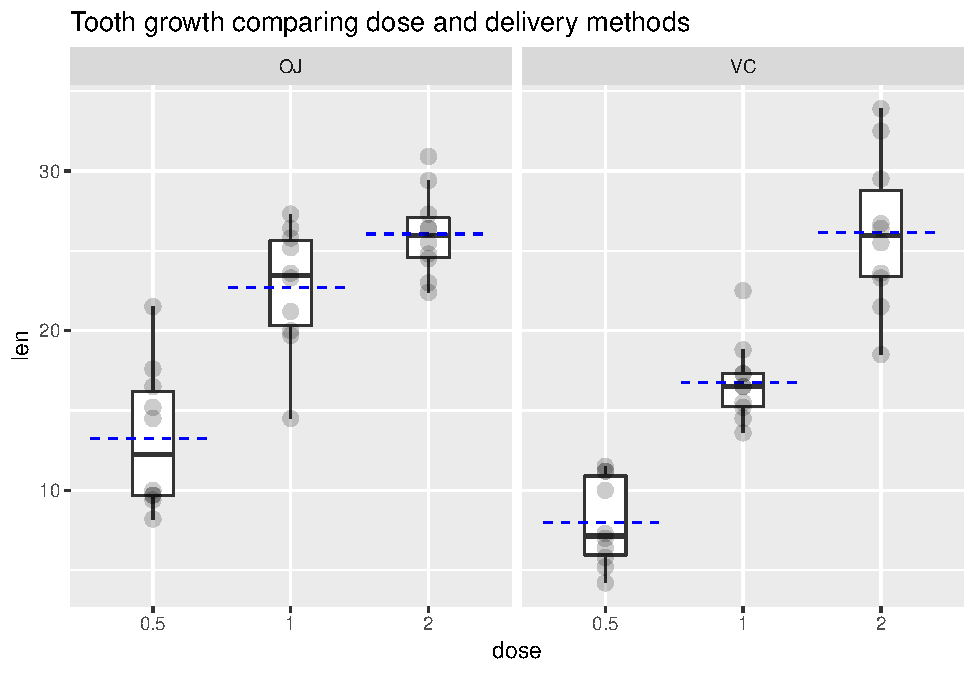
\includegraphics{Assignment_Part_2_-_Basic_Inferential_Data_Analysis_v1.1_files/figure-latex/unnamed-chunk-4-1.pdf}

\begin{Shaded}
\begin{Highlighting}[]
\CommentTok{# Show the mean for each group}
\NormalTok{tg }\OperatorTok
\StringTok{    }\KeywordTok{group_by}\NormalTok{(supp, dose) }\OperatorTok
\StringTok{    }\KeywordTok{summarise}\NormalTok{(}\DataTypeTok{mean =} \KeywordTok{mean}\NormalTok{(len))}
\end{Highlighting}
\end{Shaded}

\begin{verbatim}
## # A tibble: 6 x 3
## # Groups:   supp [?]
##   supp   dose  mean
##   <fct> <dbl> <dbl>
## 1 OJ      0.5 13.2 
## 2 OJ      1   22.7 
## 3 OJ      2   26.1 
## 4 VC      0.5  7.98
## 5 VC      1   16.8 
## 6 VC      2   26.1
\end{verbatim}

As the chart above demonstrates (note the dotted blue line represents
the mean):

\begin{itemize}
\tightlist
\item
  it looks like at the highest dose, both delivery methods result in
  similar results
\item
  at lower doses (0.5 and 1.0), orange juice delivers superior results.
\end{itemize}

\hypertarget{confidence-intervals}{%
\subsubsection{Confidence intervals}\label{confidence-intervals}}

Now lets confidence intervals and/or hypothesis tests to compare tooth
growth by supp and dose to see if our initial observations are valid.

First, we will compare the delivery methods of orange juice vs.~absorbic
acid. The mean tooth growth for samples who received orange juice is
20.6633333. The mean tooth growth for samples who received absorbic acid
is 16.9633333. The delta between these two means is 3.7.

\begin{Shaded}
\begin{Highlighting}[]
\NormalTok{t_test_result <-}\StringTok{ }\KeywordTok{t.test}\NormalTok{(len }\OperatorTok{~}\StringTok{ }\NormalTok{supp, }\DataTypeTok{paired =} \OtherTok{FALSE}\NormalTok{, }\DataTypeTok{var.equal =} \OtherTok{FALSE}\NormalTok{, }\DataTypeTok{data =}\NormalTok{ tg)}
\NormalTok{t_test_result}
\end{Highlighting}
\end{Shaded}

\begin{verbatim}
## 
##  Welch Two Sample t-test
## 
## data:  len by supp
## t = 1.9153, df = 55.309, p-value = 0.06063
## alternative hypothesis: true difference in means is not equal to 0
## 95 percent confidence interval:
##  -0.1710156  7.5710156
## sample estimates:
## mean in group OJ mean in group VC 
##         20.66333         16.96333
\end{verbatim}

As the results demonstrate, the 95\% confidence interval contains 0.
This means that although our samples showed orange juice resulted in
more growth, it would not be unusual for use to see a delta of 0, or
Orange Juice not resulting in more growth. So maybe Orange juice is not
as powerful as we thought?

Lets try comparing now a high dose vs.~a low dose, ignoring the delivery
method. The mean tooth growth for a high dose is 26.1. The mean tooth
growth for a low dose is 10.605. The delta between these two means is
15.495.

\begin{Shaded}
\begin{Highlighting}[]
\NormalTok{t_test_result <-}\StringTok{ }\KeywordTok{t.test}\NormalTok{(len }\OperatorTok{~}\StringTok{ }\NormalTok{dose, }\DataTypeTok{paired =} \OtherTok{FALSE}\NormalTok{, }\DataTypeTok{var.equal =} \OtherTok{FALSE}\NormalTok{, }\DataTypeTok{data =}\NormalTok{ tg[tg}\OperatorTok{$}\NormalTok{dose }\OperatorTok{==}\StringTok{ }\FloatTok{0.5} \OperatorTok{|}\StringTok{ }\NormalTok{tg}\OperatorTok{$}\NormalTok{dose }\OperatorTok{==}\DecValTok{2}\NormalTok{,])}
\NormalTok{t_test_result}
\end{Highlighting}
\end{Shaded}

\begin{verbatim}
## 
##  Welch Two Sample t-test
## 
## data:  len by dose
## t = -11.799, df = 36.883, p-value = 4.398e-14
## alternative hypothesis: true difference in means is not equal to 0
## 95 percent confidence interval:
##  -18.15617 -12.83383
## sample estimates:
## mean in group 0.5   mean in group 2 
##            10.605            26.100
\end{verbatim}

This time, 0 does not fall in the 95\% confidence interval. With this
knowledge, we can say that it is very unlikely that a dose of 2 is less
effective than a dose of 0.5.

\hypertarget{conclusions}{%
\subsubsection{Conclusions}\label{conclusions}}

Our analysis showed that:

\begin{itemize}
\tightlist
\item
  The orange juice method delivered higher growth than absorbic acid,
  however the difference was not statistically significant.
\item
  The higher the dose, the higher the observed tooth growth. When
  comparing a dose of 0.5 vs 2.0, the difference was statistically
  significant
\end{itemize}

From this analysis, we can conclude that under either delivery method, a
dose of 2.0 will with a high degree of confidence result in tooth
growth.


\end{document}
